\documentclass{ximera}

%\usepackage{todonotes}

\newcommand{\todo}{}

\usepackage{esint} % for \oiint
\ifxake%%https://math.meta.stackexchange.com/questions/9973/how-do-you-render-a-closed-surface-double-integral
\renewcommand{\oiint}{{\large\bigcirc}\kern-1.56em\iint}
\fi


\graphicspath{
  {./}
  {ximeraTutorial/}
  {basicPhilosophy/}
  {functionsOfSeveralVariables/}
  {normalVectors/}
  {lagrangeMultipliers/}
  {vectorFields/}
  {greensTheorem/}
  {shapeOfThingsToCome/}
  {dotProducts/}
  {partialDerivativesAndTheGradientVector/}
  {../productAndQuotientRules/exercises/}
  {../normalVectors/exercisesParametricPlots/}
  {../continuityOfFunctionsOfSeveralVariables/exercises/}
  {../partialDerivativesAndTheGradientVector/exercises/}
  {../directionalDerivativeAndChainRule/exercises/}
  {../commonCoordinates/exercisesCylindricalCoordinates/}
  {../commonCoordinates/exercisesSphericalCoordinates/}
  {../greensTheorem/exercisesCurlAndLineIntegrals/}
  {../greensTheorem/exercisesDivergenceAndLineIntegrals/}
  {../shapeOfThingsToCome/exercisesDivergenceTheorem/}
  {../greensTheorem/}
  {../shapeOfThingsToCome/}
  {../separableDifferentialEquations/exercises/}
  {vectorFields/}
}

\newcommand{\mooculus}{\textsf{\textbf{MOOC}\textnormal{\textsf{ULUS}}}}

\usepackage{tkz-euclide}
\usepackage{tikz}
\usepackage{tikz-cd}
\usetikzlibrary{arrows}
\tikzset{>=stealth,commutative diagrams/.cd,
  arrow style=tikz,diagrams={>=stealth}} %% cool arrow head
\tikzset{shorten <>/.style={ shorten >=#1, shorten <=#1 } } %% allows shorter vectors

\usetikzlibrary{backgrounds} %% for boxes around graphs
\usetikzlibrary{shapes,positioning}  %% Clouds and stars
\usetikzlibrary{matrix} %% for matrix
\usepgfplotslibrary{polar} %% for polar plots
\usepgfplotslibrary{fillbetween} %% to shade area between curves in TikZ
%\usetkzobj{all}
\usepackage[makeroom]{cancel} %% for strike outs
%\usepackage{mathtools} %% for pretty underbrace % Breaks Ximera
%\usepackage{multicol}
\usepackage{pgffor} %% required for integral for loops



%% http://tex.stackexchange.com/questions/66490/drawing-a-tikz-arc-specifying-the-center
%% Draws beach ball
\tikzset{pics/carc/.style args={#1:#2:#3}{code={\draw[pic actions] (#1:#3) arc(#1:#2:#3);}}}



\usepackage{array}
\setlength{\extrarowheight}{+.1cm}
\newdimen\digitwidth
\settowidth\digitwidth{9}
\def\divrule#1#2{
\noalign{\moveright#1\digitwidth
\vbox{\hrule width#2\digitwidth}}}




% \newcommand{\RR}{\mathbb R}
% \newcommand{\R}{\mathbb R}
% \newcommand{\N}{\mathbb N}
% \newcommand{\Z}{\mathbb Z}

\newcommand{\sagemath}{\textsf{SageMath}}


%\renewcommand{\d}{\,d\!}
%\renewcommand{\d}{\mathop{}\!d}
%\newcommand{\dd}[2][]{\frac{\d #1}{\d #2}}
%\newcommand{\pp}[2][]{\frac{\partial #1}{\partial #2}}
% \renewcommand{\l}{\ell}
%\newcommand{\ddx}{\frac{d}{\d x}}

% \newcommand{\zeroOverZero}{\ensuremath{\boldsymbol{\tfrac{0}{0}}}}
%\newcommand{\inftyOverInfty}{\ensuremath{\boldsymbol{\tfrac{\infty}{\infty}}}}
%\newcommand{\zeroOverInfty}{\ensuremath{\boldsymbol{\tfrac{0}{\infty}}}}
%\newcommand{\zeroTimesInfty}{\ensuremath{\small\boldsymbol{0\cdot \infty}}}
%\newcommand{\inftyMinusInfty}{\ensuremath{\small\boldsymbol{\infty - \infty}}}
%\newcommand{\oneToInfty}{\ensuremath{\boldsymbol{1^\infty}}}
%\newcommand{\zeroToZero}{\ensuremath{\boldsymbol{0^0}}}
%\newcommand{\inftyToZero}{\ensuremath{\boldsymbol{\infty^0}}}



% \newcommand{\numOverZero}{\ensuremath{\boldsymbol{\tfrac{\#}{0}}}}
% \newcommand{\dfn}{\textbf}
% \newcommand{\unit}{\,\mathrm}
% \newcommand{\unit}{\mathop{}\!\mathrm}
% \newcommand{\eval}[1]{\bigg[ #1 \bigg]}
% \newcommand{\seq}[1]{\left( #1 \right)}
% \renewcommand{\epsilon}{\varepsilon}
% \renewcommand{\phi}{\varphi}


% \renewcommand{\iff}{\Leftrightarrow}

% \DeclareMathOperator{\arccot}{arccot}
% \DeclareMathOperator{\arcsec}{arcsec}
% \DeclareMathOperator{\arccsc}{arccsc}
% \DeclareMathOperator{\si}{Si}
% \DeclareMathOperator{\scal}{scal}
% \DeclareMathOperator{\sign}{sign}


%% \newcommand{\tightoverset}[2]{% for arrow vec
%%   \mathop{#2}\limits^{\vbox to -.5ex{\kern-0.75ex\hbox{$#1$}\vss}}}
% \newcommand{\arrowvec}[1]{{\overset{\rightharpoonup}{#1}}}
% \renewcommand{\vec}[1]{\arrowvec{\mathbf{#1}}}
% \renewcommand{\vec}[1]{{\overset{\boldsymbol{\rightharpoonup}}{\mathbf{#1}}}}

% \newcommand{\point}[1]{\left(#1\right)} %this allows \vector{ to be changed to \vector{ with a quick find and replace
% \newcommand{\pt}[1]{\mathbf{#1}} %this allows \vec{ to be changed to \vec{ with a quick find and replace
% \newcommand{\Lim}[2]{\lim_{\point{#1} \to \point{#2}}} %Bart, I changed this to point since I want to use it.  It runs through both of the exercise and exerciseE files in limits section, which is why it was in each document to start with.

% \DeclareMathOperator{\proj}{\mathbf{proj}}
% \newcommand{\veci}{{\boldsymbol{\hat{\imath}}}}
% \newcommand{\vecj}{{\boldsymbol{\hat{\jmath}}}}
% \newcommand{\veck}{{\boldsymbol{\hat{k}}}}
% \newcommand{\vecl}{\vec{\boldsymbol{\l}}}
% \newcommand{\uvec}[1]{\mathbf{\hat{#1}}}
% \newcommand{\utan}{\mathbf{\hat{t}}}
% \newcommand{\unormal}{\mathbf{\hat{n}}}
% \newcommand{\ubinormal}{\mathbf{\hat{b}}}

% \newcommand{\dotp}{\bullet}
% \newcommand{\cross}{\boldsymbol\times}
% \newcommand{\grad}{\boldsymbol\nabla}
% \newcommand{\divergence}{\grad\dotp}
% \newcommand{\curl}{\grad\cross}
%\DeclareMathOperator{\divergence}{divergence}
%\DeclareMathOperator{\curl}[1]{\grad\cross #1}
% \newcommand{\lto}{\mathop{\longrightarrow\,}\limits}

% \renewcommand{\bar}{\overline}

\colorlet{textColor}{black}
\colorlet{background}{white}
\colorlet{penColor}{blue!50!black} % Color of a curve in a plot
\colorlet{penColor2}{red!50!black}% Color of a curve in a plot
\colorlet{penColor3}{red!50!blue} % Color of a curve in a plot
\colorlet{penColor4}{green!50!black} % Color of a curve in a plot
\colorlet{penColor5}{orange!80!black} % Color of a curve in a plot
\colorlet{penColor6}{yellow!70!black} % Color of a curve in a plot
\colorlet{fill1}{penColor!20} % Color of fill in a plot
\colorlet{fill2}{penColor2!20} % Color of fill in a plot
\colorlet{fillp}{fill1} % Color of positive area
\colorlet{filln}{penColor2!20} % Color of negative area
\colorlet{fill3}{penColor3!20} % Fill
\colorlet{fill4}{penColor4!20} % Fill
\colorlet{fill5}{penColor5!20} % Fill
\colorlet{gridColor}{gray!50} % Color of grid in a plot

\newcommand{\surfaceColor}{violet}
\newcommand{\surfaceColorTwo}{redyellow}
\newcommand{\sliceColor}{greenyellow}




\pgfmathdeclarefunction{gauss}{2}{% gives gaussian
  \pgfmathparse{1/(#2*sqrt(2*pi))*exp(-((x-#1)^2)/(2*#2^2))}%
}


%%%%%%%%%%%%%
%% Vectors
%%%%%%%%%%%%%

%% Simple horiz vectors
\renewcommand{\vector}[1]{\left\langle #1\right\rangle}


%% %% Complex Horiz Vectors with angle brackets
%% \makeatletter
%% \renewcommand{\vector}[2][ , ]{\left\langle%
%%   \def\nextitem{\def\nextitem{#1}}%
%%   \@for \el:=#2\do{\nextitem\el}\right\rangle%
%% }
%% \makeatother

%% %% Vertical Vectors
%% \def\vector#1{\begin{bmatrix}\vecListA#1,,\end{bmatrix}}
%% \def\vecListA#1,{\if,#1,\else #1\cr \expandafter \vecListA \fi}

%%%%%%%%%%%%%
%% End of vectors
%%%%%%%%%%%%%

%\newcommand{\fullwidth}{}
%\newcommand{\normalwidth}{}



%% makes a snazzy t-chart for evaluating functions
%\newenvironment{tchart}{\rowcolors{2}{}{background!90!textColor}\array}{\endarray}

%%This is to help with formatting on future title pages.
\newenvironment{sectionOutcomes}{}{}



%% Flowchart stuff
%\tikzstyle{startstop} = [rectangle, rounded corners, minimum width=3cm, minimum height=1cm,text centered, draw=black]
%\tikzstyle{question} = [rectangle, minimum width=3cm, minimum height=1cm, text centered, draw=black]
%\tikzstyle{decision} = [trapezium, trapezium left angle=70, trapezium right angle=110, minimum width=3cm, minimum height=1cm, text centered, draw=black]
%\tikzstyle{question} = [rectangle, rounded corners, minimum width=3cm, minimum height=1cm,text centered, draw=black]
%\tikzstyle{process} = [rectangle, minimum width=3cm, minimum height=1cm, text centered, draw=black]
%\tikzstyle{decision} = [trapezium, trapezium left angle=70, trapezium right angle=110, minimum width=3cm, minimum height=1cm, text centered, draw=black]


\title{Linear Forms}

\begin{document}

\begin{abstract}
constant rate
\end{abstract}
\maketitle










$\blacktriangleright$  Linear functions are those functions where the domain and range share a constant rate of change.  





Each linear function has its own constant rate of change. \\


Suppose $L$ is a linear function.  Let $a$ and $b$ be numbers in the domain of $L$.  Then $L(a)$ and $L(b)$ are the corresponding range values.

Since $L$ is a linear function, we know that $\frac{L(b) - L(a)}{b - a} = constant$.  And, this works for ANY two domain numbers.

Otherwise, it is not a linear function.







Somewhere in history, $m$ became a popular choice to represent the constant rate of change of a linear function.



\[
\frac{L(b) - L(a)}{b - a} = m
\]





No matter which two numbers you select from the domain of $L$, the rate of change always turns out to be $m$.  Each linear function has its own $m$ - its own constant rate of change.












\section{A Formula}  


Let $L$ be a linear function.  That means it has is own constant rate of change.  Let's call it $m$. \\

Let $(a, b)$ be one specific pair in $L$.\\


Let $(x, y)$ represent any other pair (all other pairs) in the function $L$. 

\begin{formula} \textbf{\textcolor{blue!55!black}{Slope}} 


Then the rate of change from $(a,b)$ to $(x, y)$ must equal $m$.


\[  \frac{y - \answer{b}}{x-\answer{a}} = m \]
\end{formula}


Clearing the denominaotr gives us the point-slope form for a line.






\begin{formula} \textbf{\textcolor{blue!55!black}{Point-Slope Form}} 


In practice, in addition to the slope, $m$, we almost always have a point on the line that is not an intercept $(a,b)$. Describing the other points on the line is much easier with the point-slope form of a line.


\[  (y - b) = m (x - a) \]
\end{formula}






Since $(a, b)$ is a pair in $L$, we know that $b = L(a)$.  And, since $(x, y)$ represents any other pair in $L$, we know that $y = L(x)$.  Replacing these in the equation for constant slope gives


\[  \frac{L(x) - L(a)}{x-a} = m \]


Clearing the denominator gives


\[  L(x) - L(a) = m (x-a) + L(a)     \]

Solving this for $L(x)$ gives

\[  L(x) = m (x-a) + L(a)     \]



\textbf{Note:} In advanced mathematics, a similar idea called \textit{linear maps} are required to include the pair $(0,0)$.  This would result in $L(0) = 0$  We will not require this for Calculus.




\begin{example} \textit{A pair and a rate-of-change}


Suppose $W$ is a linear function with constant rate of change equal to $5$ and $(3, -1)$ is one pair in $W$.  \\

Create a formula for $W$.

\begin{explanation}

The template $L(x) = m (x-a) + L(a)$ tell us that a formula for $W$ looks like 


\[  W(x) = 5 (x-3) + \left(\answer{-1}\right)     \]


\[  W(x) = 5 (x-3) - 1     \]

We could multiply this out and collect like terms and obtain the equivalent formula


\[  W(x) = \answer{5}x - \answer{16}   \]

\end{explanation}

Perhaps, we do not like $x$ as the variable for our formula.  Perhaps $v$ suits our situation better.

\[  W(v) = 5v - 16   \]


Or, $k$.

\[  W(k) = 5k - 16   \]


Or, $A$.

\[  W(A) = 5A - 16   \]


It is always advantageous to select a variable that is a nice reminder of the domain measurement.

\end{example}









\begin{example} \textit{Two Pairs}


Suppose $g$ is a linear function containing $(0, 6)$ and $(-2, -5)$.

Then the template: $L(x) = m (x-a) + L(a)$ will need a rate of change



\[  m = \frac{-5 - 6}{\answer{-2} - \answer{0}} = \frac{-11}{-2} = \frac{11}{2}  \]

A formula for $g$ is


\[  g(t) = \frac{11}{2} (t-0) + 6     \]


\[  g(t) = \frac{11}{2} t + 6    \]



\end{example}










\section{A Graph}




A linear function has a line as its graph.  The line includes a point for each pair in the function.  And, since it is a line, only two points are needed to draw the graph.  Any two distinct points will do.





\begin{example} \textit{A Line}


Let $g(k) = \frac{k}{2} - 4$ be a linear function with its natural domain. Draw a graph of $g$.


\begin{explanation}
Let's select two random domain numbers: $-4$ and $6$.  The function values at these domain numbers are $g(-4) = \answer{-6}$ and $g(6) = \answer{-1}$.  Therefore, the points $(-4, -6)$ and $(6, -1)$ are on the graph, which is a line.  We'll plot the two points and draw the line through them.


Below is the graph of $y=g(k)$.


\begin{image}
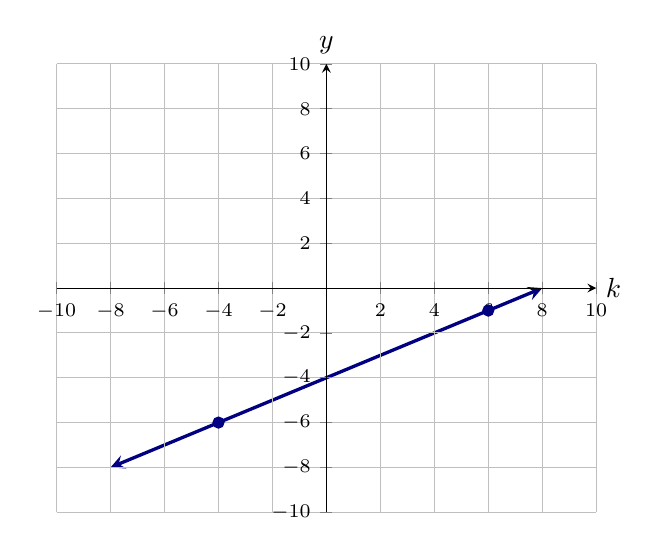
\begin{tikzpicture}
     \begin{axis}[
            	domain=-10:10, ymax=10, xmax=10, ymin=-10, xmin=-10,
            	axis lines =center, xlabel=$k$, ylabel=$y$, grid = major,
                ytick={-10,-8,-6,-4,-2,2,4,6,8,10},
                xtick={-10,-8,-6,-4,-2,2,4,6,8,10},
                ticklabel style={font=\scriptsize},
            	every axis y label/.style={at=(current axis.above origin),anchor=south},
            	every axis x label/.style={at=(current axis.right of origin),anchor=west},
            	axis on top,
          		]

        
        \addplot [draw=penColor, very thick, smooth, domain=(-8:8),<->] {0.5*x-4};

        \addplot[color=penColor,fill=penColor,only marks,mark=*] coordinates{(-4,-6)};
        \addplot[color=penColor,fill=penColor,only marks,mark=*] coordinates{(6,-1)};


    \end{axis}
\end{tikzpicture}
\end{image}


\end{explanation}

\end{example}










\begin{example} \textit{A Line}


Let $B(t)$ be a linear function.    Below is the graph of $y = B(t)$. From the graph obtain a formula for $B$.


\begin{image}
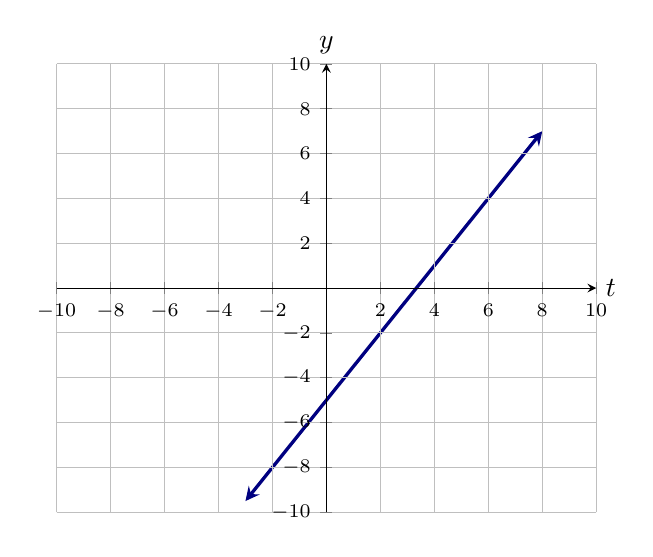
\begin{tikzpicture}
     \begin{axis}[
            	domain=-10:10, ymax=10, xmax=10, ymin=-10, xmin=-10,
            	axis lines =center, xlabel=$t$, ylabel=$y$, grid = major,
                ytick={-10,-8,-6,-4,-2,2,4,6,8,10},
                xtick={-10,-8,-6,-4,-2,2,4,6,8,10},
                ticklabel style={font=\scriptsize},
            	every axis y label/.style={at=(current axis.above origin),anchor=south},
            	every axis x label/.style={at=(current axis.right of origin),anchor=west},
            	axis on top,
          		]

        
        \addplot [draw=penColor, very thick, smooth, domain=(-3:8),<->] {(3/2)*x-5};

        %\addplot[color=penColor,fill=penColor,only marks,mark=*] coordinates{(-4,-6)};
        %\addplot[color=penColor,fill=penColor,only marks,mark=*] coordinates{(6,-1)};


    \end{axis}
\end{tikzpicture}
\end{image}

\begin{explanation}

From the graph, we can approximate the points $(0, -5)$ and $(3.3, 0)$.  These give a slope of

\[  slope = \frac{0 - \left(\answer{-5}\right)}{\answer{3.3} - 0} = \frac{5}{3.3} (\approx 1.5)     \]


This would give the formula $B(t) = \frac{5}{3.3} (t - 0) - 5 = \frac{5}{3.3} t - 5$

\end{explanation}

\end{example}


We used the point $(0, -5)$ to create the equation.  We could also have used $(3.3,0)$.



$B(t) = \frac{5}{3.3} (t - 3.3) - 0 = \frac{5}{3.3} t - \frac{5}{3.3}\cdot 3.3 = \frac{5}{3.3} t -  5$ \\


Same equation.  You can use any point on the line.















\section{Linear Equations}


\begin{definition} \textbf{\textcolor{green!50!black}{Linear Equation}} \\


A \textbf{linear equation in $x_1$ and $x_2$} is an equation that is equivalent to 

\[
a \, x_1 + b \, x_2 + c = 0
\]


$x_1$ and $x_2$ are the \textbf{variables}.

$a$ and $b$ are constants called \textbf{coefficients}.

$c$ is called the \textbf{constant term}.

\end{definition}










\begin{definition} \textbf{\textcolor{green!50!black}{Solution}} \\


A \textbf{solution} to the linear equation  $a \, x_1 + b \, x_2 + c = 0$ is an ordered pair of numbers that \textbf{satisfy} the equation.


\end{definition}

\begin{notation}


We often write solution pairs as an ordered pair: $(A, B)$. \\


One of the solution numbers is designated for $x_1$ and one is designated for $x_2$.  (That is what ordered means.) Upon substituting these numbers into the equation for $x_1$ and $x_2$, the resulting statement is a true statement, i.e. the equation is \textit{satisfied}. \\

If the order is not understood, then we might write $(x_1, x_2) = (A, B)$.


\end{notation}





With the order understood, each solution pair can be interpreted as coordinates for a point on the Cartesian plane and plotted as a dot.




\begin{example}






Consider the linear equation  $3 t + 2 y = 12$.


Let's select $t$ to be the first variable and $y$ the second variable.

With this agreement, $(4, 0)$ is a solution to the equation.   $(4,0)$ can be viewed as a point and plotted as a dot on the Cartesian plane.



\begin{image}
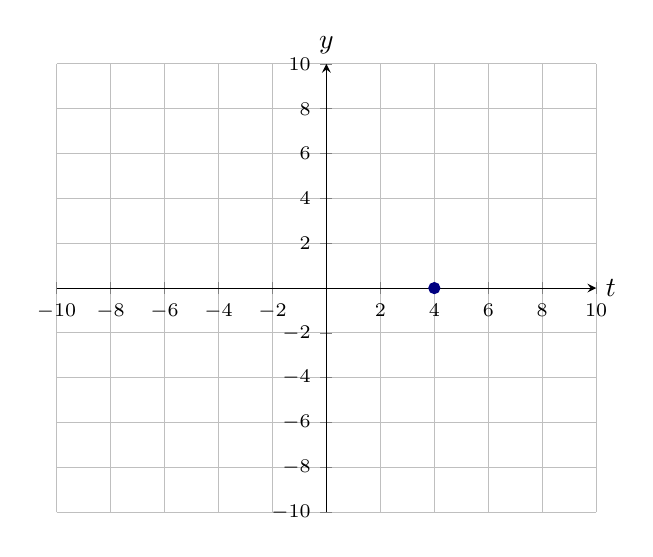
\begin{tikzpicture}
     \begin{axis}[
                domain=-10:10, ymax=10, xmax=10, ymin=-10, xmin=-10,
                axis lines =center, xlabel=$t$, ylabel=$y$, grid = major,
                ytick={-10,-8,-6,-4,-2,2,4,6,8,10},
                xtick={-10,-8,-6,-4,-2,2,4,6,8,10},
                ticklabel style={font=\scriptsize},
                every axis y label/.style={at=(current axis.above origin),anchor=south},
                every axis x label/.style={at=(current axis.right of origin),anchor=west},
                axis on top,
                ]

        
        %\addplot [draw=penColor, very thick, smooth, domain=(-3:8),<->] {(3/2)*x-5};

         \addplot[color=penColor,fill=penColor,only marks,mark=*] coordinates{(4,0)};


    \end{axis}
\end{tikzpicture}
\end{image}







If we plot a dot for each and every solution pair for the equation, then we obtain the graph of the equation.  






\begin{image}
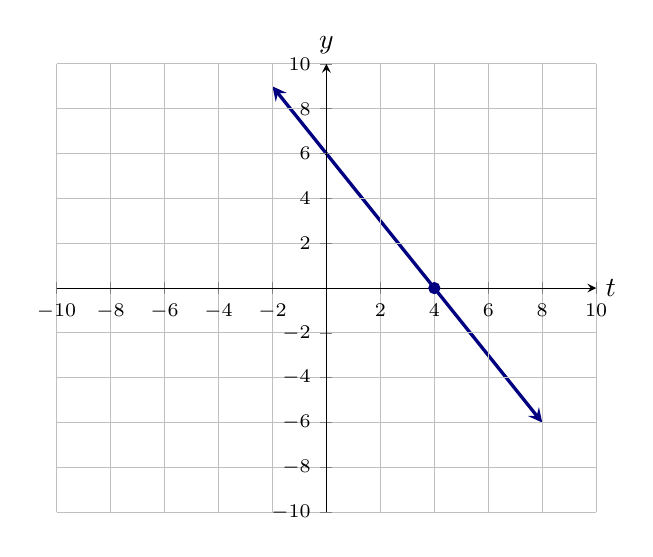
\begin{tikzpicture}
     \begin{axis}[
                domain=-10:10, ymax=10, xmax=10, ymin=-10, xmin=-10,
                axis lines =center, xlabel=$t$, ylabel=$y$, grid = major,
                ytick={-10,-8,-6,-4,-2,2,4,6,8,10},
                xtick={-10,-8,-6,-4,-2,2,4,6,8,10},
                ticklabel style={font=\scriptsize},
                every axis y label/.style={at=(current axis.above origin),anchor=south},
                every axis x label/.style={at=(current axis.right of origin),anchor=west},
                axis on top,
                ]

        
        \addplot [draw=penColor, very thick, smooth, domain=(-2:8),<->] {(-1.5)*(x-4)};

         \addplot[color=penColor,fill=penColor,only marks,mark=*] coordinates{(4,0)};


    \end{axis}
\end{tikzpicture}
\end{image}

The graph of a linear equation is a line, which can be drawn using only two points from two solution pairs.














\end{example}

Graphs of lines don't care which axis is ``vertical'' and which axis is ``horizontal''.  The graph is just a collection of points whose coordinates satisfy the linear equation.  The situation changes once we wish to interpret one of the variables as a function of the other variable. \\




Once we designate one of the variables as the dependent variable or the function, then its axis becomes the ``vertical'' axis.  The other axis measures the independent variable and represents the domain of the function. \\


Except for vertical lines, all lines are graphs of linear functions. \\



\begin{explanation}
If we interpret the first or left variable as representing domain values and the second or right variable as representing function values, then linear equations describe linear functions.  We can solve the equation for the function variable to obtain a formula.



In the example above, $3 t + 2 y = 12$ can be rewritten as $y = \answer{\frac{-3}{2}} t + \answer{6}$.

To emphasize that we are now thinking in terms of functions, we might write $y(t) = \tfrac{-3}{2} t + 6$.




We could just as easily have chosen $y$ as the domain variable and $t$ as the function variable.  In this case, $3 t + 2 y = 12$ can be rewritten as $t = \answer{\frac{-2}{3}} y + \answer{4}$.  We might write this as $t(y) = \tfrac{-2}{3} y + 4$




In either case, the function formula matches the ``$y = m \, x + b$'' template.  $\answer{m}$ is the slope of the line as well as the rate of change of the function.


\end{explanation}










\begin{center}
\textbf{\textcolor{green!50!black}{ooooo=-=-=-=-=-=-=-=-=-=-=-=-=ooOoo=-=-=-=-=-=-=-=-=-=-=-=-=ooooo}} \\

more examples can be found by following this link\\ \link[More Examples of Linear Functions]{https://ximera.osu.edu/csccmathematics/precalculus1/precalculus1/linearFunctions/examples/exampleList}

\end{center}





\end{document}
